\documentclass[11pt]{exam}
\usepackage[margin=1in]{geometry}
\pagestyle{plain}
\usepackage{amsmath,amsfonts,amssymb,amsthm,enumerate}
\usepackage{multicol}
\usepackage[]{graphicx}
\usepackage{hyperref}
\usepackage{tikz}
\usepackage{pgfplots}
\usepackage{subfigure}
\usepackage[final]{pdfpages}


\everymath{\displaystyle}

\addtolength{\footskip}{2\baselineskip} % to lower the page numbers
\title{\vspace{-0.5in} Math 115 \\ Worksheet Section 5.3}
\date{}


% \theoremstyle{definition}
% \newtheorem{problem}{Problem}
\renewcommand{\questionlabel}{\textbf{Problem~\thequestion.}}
%\printanswers

\begin{document}
\maketitle
\vspace{-0.75in}
\section*{Warm-up question}
\noindent
What does the Fundamental Theorem of Calculus say?
\begin{solution}
 If \(f\) is continuous on the interval \([a,b]\) and \(f(t) =
 F'(t)\), then \[
   \int_a^b f(t) dt = F(b) - F(a) \,.
 \]
\end{solution}
\vspace{4em}
\begin{questions}
  \question 
    \begin{multicols}{2}
\begin{enumerate}[(a)]
\item Differentiate $x^3+x$.
\item Compute $\displaystyle\int_0^2(3x^2+1)dx$
\item Differentiate $e^{x^2}$.
\item Compute $\displaystyle\int_0^1 xe^{x^2}dx$
\end{enumerate}	
\end{multicols}
\begin{solution}
  \begin{enumerate}[(a)]
  \item \(3x^2+1\)
  \item Since \(x^3+x\) is an anti-derivative of \(3x^2+1\), we get
    \(\int_0^2 (3x^2+1) dx = 2^3+2 - (0^3+0)\). 
  \item \(2x e^{x^2}\)
  \item Since \(\frac{1}{2} e^{x^2}\) is an anti-derivative of \(x
    e^{x^2}\), we get \(\int_0^1 x e^{x^2} dx =
    \frac{1}{2}e^{1^2}-\frac{1}{2}e^{0^2} = \frac{1}{2}\).
  \end{enumerate}
\end{solution}
  \question Explain in words what these integrals represent, with units.
    \begin{parts}
    \part \(\int_0^6 a(t) dt\) where \(a(t)\) is acceleration in
      km/hr\({}^2\) and \(t\) is time in hours.
    \part \(\int_{2005}^{2011} f(t) dt\) where \(f(t)\) is the rate at
      which the world's population is growing in year \(t\), in
      billion people per year.
    \end{parts}
    \begin{solution}
      \begin{enumerate}[(a)]
      \item The net change in velocity in the first \(6\) hours is
        \(\int_0^6 a(t) dt\).
      \item The world's population grew by \(\int_{2005}^{2011} f(t)
        dt\) from 2005 to 2011.
      \end{enumerate}
    \end{solution}
   \question Pollution is removed from a lake on day \(t\) at a rate
     of \(f(t)\) kg/day.
     \begin{parts}
     \part Explain the meaning of the statement \(f(12) = 500\).
     \part If \(\int_5^{15} f(t) dt = 4000\), give the units of the
       bounds of integration (\(5\) and \(15\)), and the units for the
       result of the integral.
     \part Give the meaning of \(\int_5^{15} f(t) dt = 4000\).
     \end{parts}
     \begin{solution}
       \begin{enumerate}[(a)]
       \item On day 12, pollution is removed at \(500\) kg/day.
       \item 5 and 15 are in units of days and 4000 is in units of kg.
       \item Between day 5 and day 15, \(4000\) kg of pollution was removed.
       \end{enumerate}
     \end{solution}
\question 
  \begin{multicols}{2}
    \begin{parts}
    \part What is the derivative of \(\sin t\)?
    \part The velocity of a particle at time \(t\) is
      \(v(t) = \cos t\). Use the Fundamental Theorem of Calculus to
      find the total distance traveled by the particle between \(t=0\)
      and \(t = \pi/2\)
    \part Does your answer make sense with the graph of \(\cos t\)?
    \end{parts}
    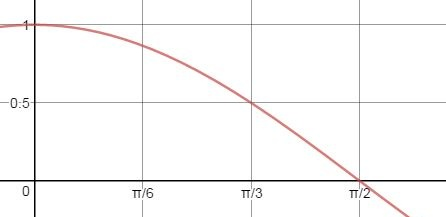
\includegraphics[width=3in]{cosine.jpg}
  \end{multicols}
  \begin{solution}
    \begin{enumerate}[(a)]
    \item \(\cos t\)
    \item Total distance traveled will be \(\int_0^{\pi/2} \cos (t) dt =
      \sin(\pi/2) - \sin(0) = 1\) by the Fundamental Theorem of Calculus.
    \item Remembering that \(\pi/6 \approx 1/2\), it seems that the
      total area below the curve is around 1.
    \end{enumerate}
  \end{solution}
\question Use the given graph to answer the following:

\begin{multicols}{2}

(a) Which is larger, $f(0)$ or $f(1)$?

\vskip2ex
(b) List the following in increasing order: 
$\hspace*{1cm}\displaystyle\frac{f(4)-f(2)}{2}, \quad f(3)-f(2), \quad f(4)-f(3).$
\vskip3ex


\columnbreak
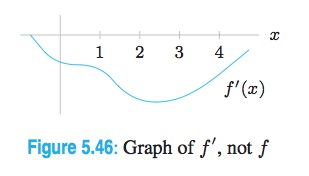
\includegraphics[width=2.8in]{no3334graph.jpg}
\end{multicols}
\begin{solution}
  \begin{enumerate}[(a)]
  \item \(f(0) > f(1)\) since \(f(x)\) is decreasing from 0 to 1
    (because \(f'(x) < 0\) from 0 to 1).
  \item Each of these quantities can be rewritten as a definite
    integral \[
      \frac{f(4)-f(2)}{2} = \frac{1}{2} \int_2^4 f'(x) dx \qquad
      f(3)-f(2) = \int_2^3 f'(x) dx \qquad f(4) - f(3) =
      \int_3^4 f'(x) dx
    \]
    Thus, we can compare the various (signed) areas under the graph to see \[
      \int_2^3 f'(x) < \frac{1}{2} \int_2^4 f'(x) < \int_3^4 f'(x) dx
    \]
    and therefore, \[
      f(3) - f(2) < \frac{f(4)-f(2)}{2} < f(4) - f(3)
    \]
  \end{enumerate}
\end{solution}
\question Water is leaking out of a tank at a rate of \(R(t)\)
  gallons/hour, graphed below, where \(t\) is measured in hours.
  \begin{multicols}{2}
    \begin{parts}
    \part Write a definite integral that expresses the total amount of
      water that leaks out in the first two hours.
    \part In the figure, shade the region whose area represents the
      total amount of water that leaks out in the first two hours.
    \part Give an upper and lower estimate of the total amount of
      water that leaks out in the first two hours.
    \end{parts}
    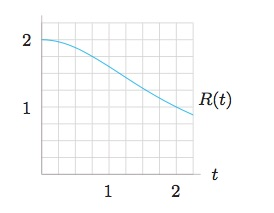
\includegraphics[width=2.7in]{no21graph.jpg}
  \end{multicols}
  \begin{solution}
    \begin{enumerate}[(a)]
    \item \(\int_0^2 R(t) dt\)
    \item 
    \item Since the function \(R(t)\) is decreasing, we can do this
      with Riemann sums. The left-hand sum will be an overestimate and
      the right-hand sum will be an underestimate. For instance, if we
      take \(n=3\) rectangles, we will have an overestimate of \[
        \frac{2}{3}\left( 2 + 1.75+1.25 \right) = \frac{10}{3} \approx 3.33
      \]
      and an underestimate of \[
       \frac{2}{3}\left( 1.75 + 1.25 + 0.9 \right) = 2.6
      \]
    \end{enumerate}
  \end{solution}
\question Consider the integral $\displaystyle\int_{-1}^1 \sqrt{1-x^2} \, dx$ and $\displaystyle G(x) = \frac{1}{2}\left(x\sqrt{1-x^2}+\arcsin(x)\right)$.
\begin{enumerate}[(a)]
	\item Sketch the graph of the function $y = \sqrt{1-x^2}$ on the interval $[-1,1]$.
	\item Find the exact value of the integral using your knowledge of areas.
	\item Show that $G'(x)=\sqrt{1-x^2}$.
	\item Does your answer in part (b) agree with the fundamental theorem of calculus? 
\end{enumerate}	
\begin{solution}
  \begin{enumerate}[(a)]
  \item 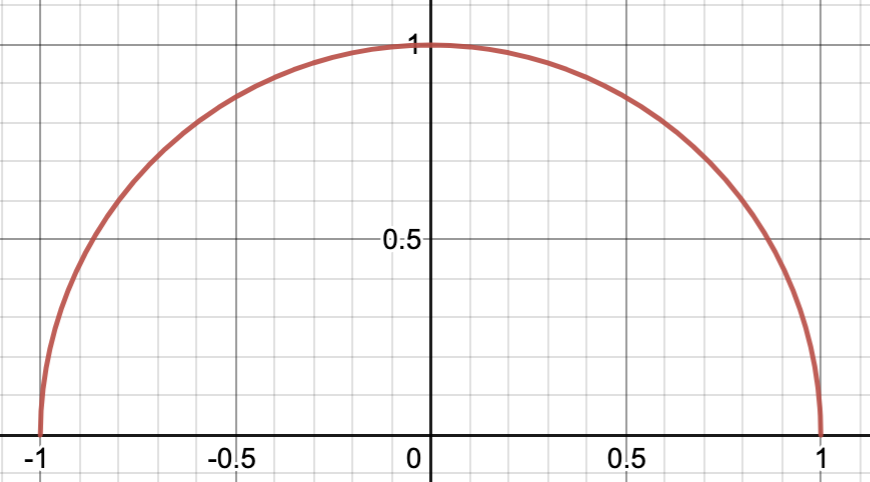
\includegraphics[scale=0.5]{half-circle-graph}
  \item \(\int_{-1}^1 \sqrt{1-x^2} dx = \frac{\pi}{2}\) since the
    equation is that of a half-circle
  \item Using our derivative rules, we compute \[
      G'(x) = \frac{1}{2}\left( 1 \cdot \sqrt{1-x^2} - 
        x \cdot \frac{x}{\sqrt{1-x^2}} + \frac{1}{\sqrt{1-x^2}} \right) 
    \]
    Then, giving a common denominator and simplifying, we get \[
      G'(x) = \frac{1-x^2-x^2+1}{2 \sqrt{1-x^2}} = \sqrt{1-x^2}
    \]
  \item The Fundamental Theorem of Calculus tells us \[
      \int_{-1}^1 \sqrt{1-x^2} dx = G(1) - G(-1) = \frac{1}{2}\arcsin(1) -
      \frac{1}{2}\arcsin(-1) = \frac{\pi}{4} - \left( -\frac{\pi}{4}
      \right) = \frac{\pi}{2}
    \]
    This agrees with the answer in part (a).
  \end{enumerate}
\end{solution}
\question Below is a table with some values of a twice differentiable function $f(x)$	and its derivative.
	$$\begin{array}{|c||c|c|c|c|}
	\hline
	x & -1 & 0 & 3 & 5 \\
	\hline
	f(x) & 3 & 5 & 7 & 3 \\
	\hline
	f'(x) & 1 & -3 & 6 & 2\\
	\hline	
	\end{array}$$
\begin{enumerate}[(a)]
	\item Find $\displaystyle\int_{-1}^3 f'(x) \, dx$.
	\item If $\displaystyle\int_{0}^2 f''(x) \, dx = 5$, find $f'(2)$.
	\item Assume $f$ is concave up on the interval $[0,3]$. What is the area between the graph of $f''$ and the $x$-axis on the interval $[0,3]$?
	\item Find $\displaystyle\int_0^{\frac{\pi}{2}} (f'(x)\cos(x) - f(x) \sin(x)) \, dx$.
\end{enumerate}
\begin{solution}
  \begin{enumerate}[(a)]
  \item \[
      \int_{-1}^3 f'(x) dx = f(3)-f(-1) = 7-3 = 4
    \]
  \item \[
      5 = \int_0^2 f''(x) dx = f'(2) - f'(0) \implies f'(2) = 5+f'(0)
      = 5+5 = 10
    \]
  \item If \(f\) is concave up on \([0,3]\), then \(f''(x) > 0\) on
    \([0,3]\), so the area between the graph of \(f''\) and the
    \(x\)-axis on \([0,3]\) is \[
      \int_0^3 f''(x) dx = f'(3) - f'(0) = 6 - (-3) = 9
    \]
  \item We note that \(g(x) = f(x)\cos(x)\) satisfies \(g'(x) = f'(x)
    \cos(x) - f(x)\sin(x)\) and thus \[
      \int_0^{\frac{\pi}{2}} (f'(x)\cos(x) - f(x) \sin(x)) \, dx =
      f(\pi/2)\cos(\pi/2) - f(0)\cos(0) = -5
    \]
  \end{enumerate}
\end{solution}
\pagebreak
\question (Winter 2017 Final Exam) % problem 3
	Virgil, Duncan, Jasper and Zander are all watching a toy
        wind-up mouse move across the floor. The toy is placed on the
        floor 2.3 meters away from Virgil, and it moves in a straight
        line directly away from Virgil at a strictly decreasing
        velocity. Below are some values of $v(t)$, the velocity of the
        toy mouse (m/s), $t$ seconds after the toy is placed on the
        floor, where a positive velocity corresponds to the toy moving
        away from Virgil.
        
        \begin{center}
          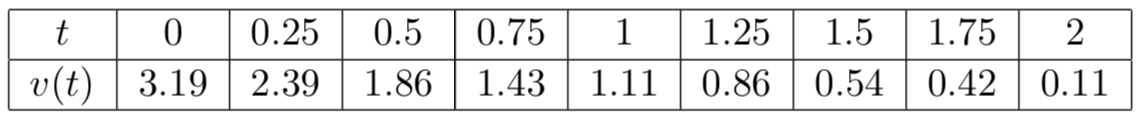
\includegraphics[scale=0.5]{Figures/table}
        \end{center}
\vspace{-1em}
\begin{enumerate}[(a)]
	\item Estimate the value of $\displaystyle\int_{0.25}^{1.75} v(t) \, dt$ using a left-hand Riemann sum with $\Delta t = 0.5$. Be sure to write down all the terms. Is your estimation an overestimate or an underestimate?
	\item  How often should the values of $v(t)$ be measured in order to find upper and lower estimates for  $\displaystyle\int_{0.25}^{1.75} v(t) \, dt$ that are within 0.1 m of the actual value?
	\item Find the value of $\displaystyle\int_{0.5}^{1.25} v'(t) \, dt$.
	\item Which of the following represents how much the distance from the toy mouse to Virgil increases during the 2$^{\textrm{nd}}$ second after it has been placed on the floor? Circle the one best answer.
	\begin{multicols}{3}
	\begin{enumerate}[(i)]
		\item $2.3 - \displaystyle\int_1^2 v(t) \, dt$
		\item $2.3 - \displaystyle\int_1^2 v'(t) \, dt$
		\item $\displaystyle\int_1^2 v(t) \, dt - \displaystyle\int_0^1 v(t) \, dt$
		\item $\displaystyle\int_1^2 v(t) \, dt$
		\item $\displaystyle\int_1^2 v'(t) \, dt$
		\item $v(2) - v(1)$
	\end{enumerate}
	\end{multicols}
\end{enumerate}
\begin{solution}
  See \href{https://dhsp.math.lsa.umich.edu/exams/115exam3/w17/s3.pdf}{https://dhsp.math.lsa.umich.edu/exams/115exam3/w17/s3.pdf}
\end{solution}
\question (Fall 2014 Final Exam)
A professor delivers a $60$ minute lecture on the general theory of relativity. One eager undergraduate student takes notes by typing what the professor says, word for word. Unfortunately the student cannot always type as quickly as the professor is speaking. The graph below shows the professor's speaking rate $p(t)$ (dashed) in words per minute (wpm) and the student's typing rate $u(t)$ (solid), also in words per minute (wpm).

\begin{center}
  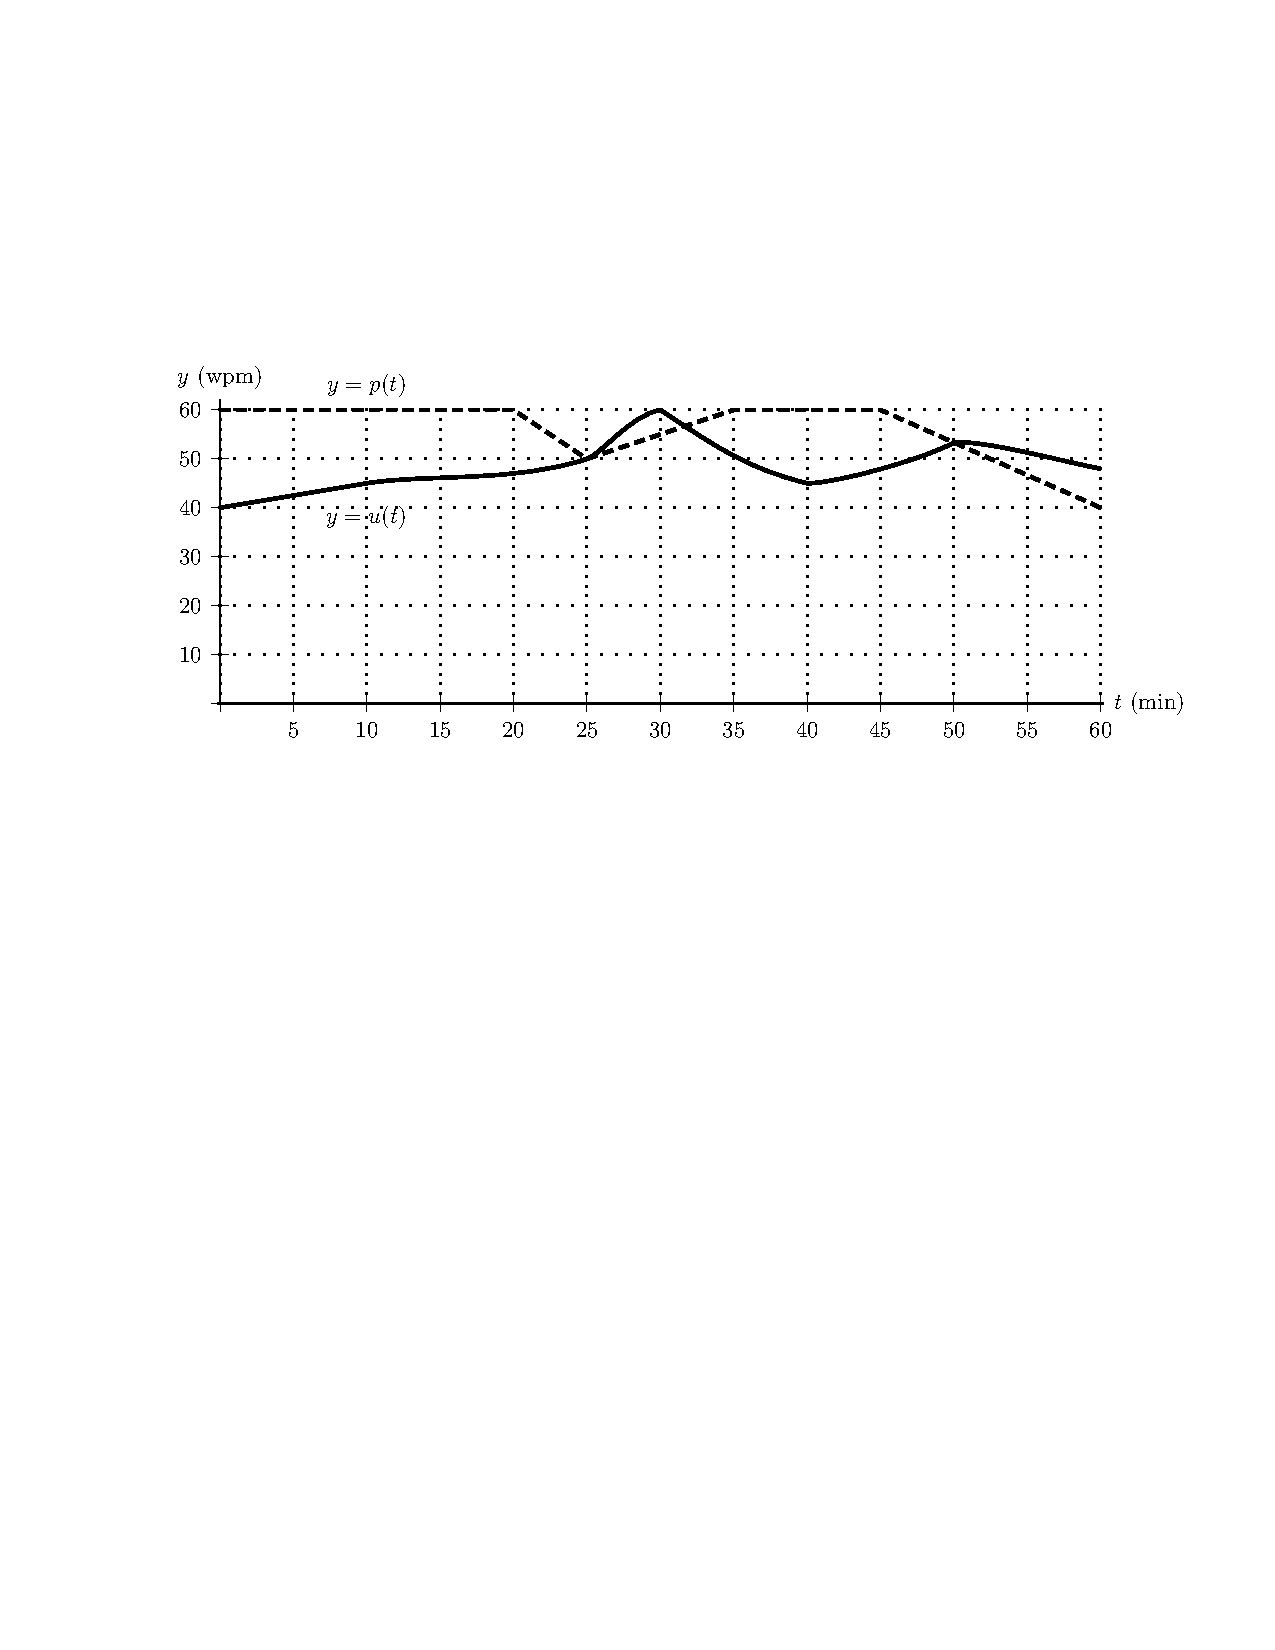
\includegraphics[width=7cm,height=3cm]{Figures/fig2.pdf}
\end{center}
\begin{enumerate}[(a)]
	\item How many minutes after the start of the lecture is the student typing most quickly?
	\item Write a definite integral equal to the number of words the student types between the start of the lecture and the time the professor reaches the $600$th {\bf word} of his lecture. 
	%You do not need to evaluate the integral.
	\item How many minutes after the start of the lecture is the student furthest behind in typing up the lecture? (When is the difference between the total number of words the professor has spoken and the total number of words the student has typed the greatest?)
\end{enumerate}
\begin{solution}
  See \href{https://dhsp.math.lsa.umich.edu/exams/115exam3/f14/s7.pdf}{https://dhsp.math.lsa.umich.edu/exams/115exam3/f14/s7.pdf}
\end{solution}
\pagebreak
\question (Fall 2011 Final Exam)
The graph below shows the rate of snow melt and snowfall on Mount Arvon, the highest peak in Michigan, during a day in April of last year. The function $m(t)$ (solid curve) is rate of snow melt, in inches per hour, $t$ hours after the beginning of the day. The function $p(t)$ (dashed curve) is the snowfall rate in inches per hour $t$ hours after beginning of the day. There were $18$ inches of snow on the ground at the beginning of the day.

\begin{center}
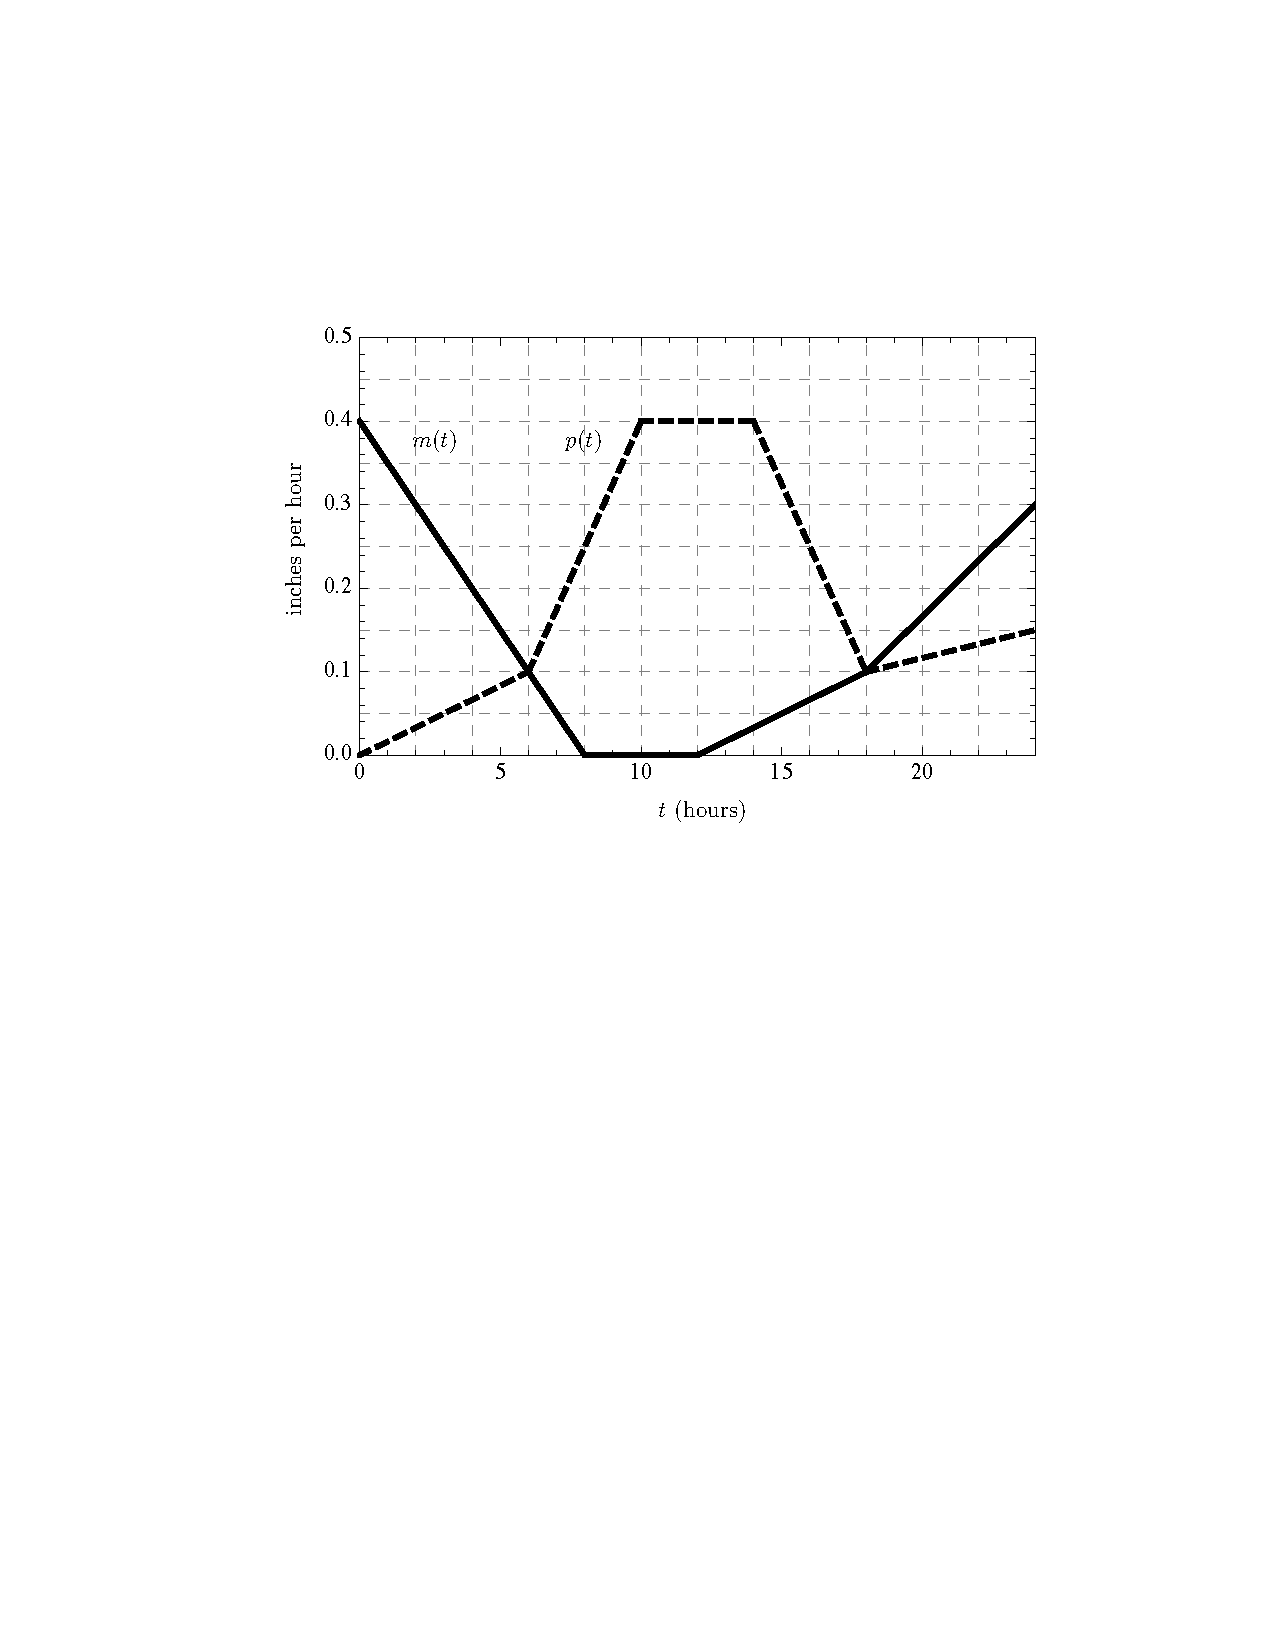
\includegraphics[width=7cm,height=5cm]{Figures/fig1.pdf}
\end{center}
\begin{enumerate}[(a)]
	\item Over what time period(s) was the snowfall rate greater than the snow melt rate?
	\item When was the amount of snow on Mount Arvon increasing the fastest?
	\item When was the amount of snow on Mount Arvon decreasing the fastest?
	\item When was the amount of snow on Mount Arvon the greatest? Explain.
	\item How much snow was there on Mount Arvon at the end of the day (at $t=24$)?
\end{enumerate}
\begin{solution}
  See \href{https://dhsp.math.lsa.umich.edu/exams/115exam3/f11/s3.pdf}{https://dhsp.math.lsa.umich.edu/exams/115exam3/f11/s3.pdf}
\end{solution}
\question (Winter 2018 Final Exam) % problem 2
	There were 3 trillion trees in the world in the year 2000.
\begin{itemize}
	\item Since the year 2000, a group of environmentalists have recorded the number of trees lost in the world due to natural causes or due to human activities. Let $C(t)$ be the rate at which the number of trees decreases due to any of these causes, t years after the year 2000, in trillions of trees per year.
	\item At the same time, some governments and other organizations plant new trees to increase the number of trees in the world. The group is also measuring the rate $P(t)$ at which the trees are being planted, t years after the year 2000, in trillions of trees per year.
\end{itemize}
Throughout this question, you may assume that the functions $C(t)$ and $P(t)$ describe the only changes to the number of trees in the world.
\begin{enumerate}[(a)]
	\item Find an expression for the total number of trees in the world (in trillions) in the year 2005.
	\item Find an expression for the average rate at which the trees were being planted (in trillions of trees per year) between the years 2002 and 2009.
	\item Write a practical interpretation of the statement $\displaystyle\int_{13}^{17} C(t) \, dt = 0.05$. Your answer must be a complete sentence.
\end{enumerate}
\begin{solution}
  See \href{https://dhsp.math.lsa.umich.edu/exams/115exam3/w18/s2.pdf}{https://dhsp.math.lsa.umich.edu/exams/115exam3/w18/s2.pdf}
\end{solution}
\end{questions}
\end{document}
%%% Local Variables:
%%% mode: latex
%%% TeX-master: t
%%% End:
